%%%%%%%%%%%%%%%%%%%%%%%%%%%%%%%%%%%%%%%%%
% Beamer Presentation
% LaTeX Template
% Version 1.0 (10/11/12)
%
% License:
% CC BY-NC-SA 3.0 (http://creativecommons.org/licenses/by-nc-sa/3.0/)
%
%%%%%%%%%%%%%%%%%%%%%%%%%%%%%%%%%%%%%%%%%

%----------------------------------------------------------------------------------------
%	PACKAGES AND THEMES
%----------------------------------------------------------------------------------------

\documentclass{beamer}

\usepackage{polski}
\usepackage[utf8]{inputenc}

\mode<presentation> {

% The Beamer class comes with a number of default slide themes
% which change the colors and layouts of slides. Below this is a list
% of all the themes, uncomment each in turn to see what they look like.

%\usetheme{default}
%\usetheme{AnnArbor}
%\usetheme{Antibes}
%\usetheme{Bergen}
%\usetheme{Berkeley}
%\usetheme{Berlin}
%\usetheme{Boadilla}
%\usetheme{CambridgeUS}
%\usetheme{Copenhagen}
%\usetheme{Darmstadt}
%\usetheme{Dresden}
%\usetheme{Frankfurt}
%\usetheme{Goettingen}
%\usetheme{Hannover}
%\usetheme{Ilmenau}
%\usetheme{JuanLesPins}
%\usetheme{Luebeck}
\usetheme{Madrid}
%\usetheme{Malmoe}
%\usetheme{Marburg}
%\usetheme{Montpellier}
%\usetheme{PaloAlto}
%\usetheme{Pittsburgh}
%\usetheme{Rochester}
%\usetheme{Singapore}
%\usetheme{Szeged}
%\usetheme{Warsaw}

% As well as themes, the Beamer class has a number of color themes
% for any slide theme. Uncomment each of these in turn to see how it
% changes the colors of your current slide theme.

%\usecolortheme{albatross}
%\usecolortheme{beaver}
%\usecolortheme{beetle}
%\usecolortheme{crane}
%\usecolortheme{dolphin}
%\usecolortheme{dove}
%\usecolortheme{fly}
%\usecolortheme{lily}
%\usecolortheme{orchid}
%\usecolortheme{rose}
%\usecolortheme{seagull}
%\usecolortheme{seahorse}
%\usecolortheme{whale}
%\usecolortheme{wolverine}

%\setbeamertemplate{footline} % To remove the footer line in all slides uncomment this line
%\setbeamertemplate{footline}[page number] % To replace the footer line in all slides with a simple slide count uncomment this line

%\setbeamertemplate{navigation symbols}{} % To remove the navigation symbols from the bottom of all slides uncomment this line
}

\usepackage{graphicx} % Allows including images
\usepackage{booktabs} % Allows the use of \toprule, \midrule and \bottomrule in tables
\usepackage{outlines}
%\usepackage{algorithm}% http://ctan.org/pkg/algorithms
\usepackage{algpseudocode}% http://ctan.org/pkg/algorithmicx

%----------------------------------------------------------------------------------------
%	TITLE PAGE
%----------------------------------------------------------------------------------------

\title[]{Harmonogramowanie zadań wielomaszynowych z przezbrojeniami} % The short title appears at the bottom of every slide, the full title is only on the title page

\author{Michał Zimniak, Norbert Januszek} % Your name
\institute[] % Your institution as it will appear on the bottom of every slide, may be shorthand to save space
{
Uniwersytet Wrocławski \\ % Your institution for the title page
\medskip
\textit{zimniak.michal@gmail.com} % Your email address
\textit{traspie@wp.pl}
}
\date{\today} % Date, can be changed to a custom date

\begin{document}

\begin{frame}
\titlepage % Print the title page as the first slide
\end{frame}

%
%\begin{frame}
%\frametitle{Overview} % Table of contents slide, comment this block out to remove it
%\tableofcontents % Throughout your presentation, if you choose to use \section{} and %\subsection{} commands, these will automatically be printed on this slide as an overview of your %presentation
%\end{frame}
%
%----------------------------------------------------------------------------------------
%	PRESENTATION SLIDES
%----------------------------------------------------------------------------------------


\begin{frame}
\frametitle{Wstęp}
Będziemy rozpatrywać problem szeregowania zadań wielomaszynowych z przezbrojeniami maszyn.
Chcemy zminimalizować iloczyn liczby użytych maszyn i długość wykonywania wszystkich zadań.
\end{frame}

\begin{frame}
    \frametitle{Specyfikacja problemu}
    Dane wejściowe
    \begin{outline}
        \1 Zbiór zadań $\mathcal{J}=\{1,2,\dots,n\}$
        \2 Zadanie $i\in\mathcal{J}$ wymaga jednocześnie $size_i$ maszyn przez $p_i>0$
        jednostek czasu.
        
        \1 Zbiór maszyn $\mathcal{M}=\{1,2,\dots,m\}$
        \2 Maszyny $l,k\in\mathcal{M}$ nazywamy sąsiednimi, jeżeli $k=l+1$ lub $k=l-1$.
        \2 Przez $s_{i,j}$ oznaczamy czas przezbrojenia pomiędzy zadaniem $i$, a zadaniem $j$.
    \end{outline}
\end{frame}

\begin{frame}
    \frametitle{Specyfikacja problemu}
    Założenia
    \begin{outline}
        \1 Żadna maszyna nie może wykonywać więcej niż jedno zadanie w danym momencie.
        \1 Wykonywanie zadania nie może być przerwane.
        \1 Każde zadanie jest wykonywane na wymaganej liczbie sąsiednich maszyn.
        \1 Pomiędzy kolejno wykonywanymi zadaniami należy wykonać przezbrojenie maszyny.
        \1 Zakładamy, że liczba maszyn $m\ge\max\{size_i : i\in\mathcal{J}\}$, czyli jesteśmy
        w stanie wykonać każde zadanie.
    \end{outline}
\end{frame}

\begin{frame}
    \frametitle{Specyfikacja problemu}
    Rozwiązanie
    \begin{outline}
        \1 Należy dla każdego zadania wyznaczyć podzbiór maszyn oraz momentów rozpoczęcia jego wykonywania spełniając wymienione ograniczenia, tak żeby zminimalizować iloczyn liczby
        użytych maszyn i długość wykonywania wszystkich zadań.
    \end{outline}
    
    
    Rozwiązanie może być reprezentowane przez parę $\Theta=(\mathcal{Q},\mathcal{S})$ taką, że:
    \begin{outline}
        \1 $\mathcal{Q}=(\mathcal{Q}_1,\mathcal{Q}_2,\dots,\mathcal{Q}_n)$, gdzie 
        $\mathcal{Q}_i \subseteq \mathcal{M}$
        to zbiór maszyn na których będzie wykonywane zadanie $i\in\mathcal{J}$.
        \1 $\mathcal{S}=(\mathcal{S}_{1,1},\dots,\mathcal{S}_{1,m},\mathcal{S}_{2,1},
        \dots,\mathcal{S}_{2,m},\dots,\mathcal{S}_{n,1},\dots,\mathcal{S}_{n,m})$, gdzie
        $\mathcal{S}_{i,j}$ jest momentem rozpoczęcia wykonywania zadania $i$ na maszynie $j$.
        Jeżeli $j\notin\mathcal{Q}_i$ to $\mathcal{S}_{i,j}=-\infty$.
    \end{outline}
    
\end{frame}

\begin{frame}
    \frametitle{Specyfikacja problemu}
    Funkcja celu
    \begin{outline}
        \1 $F(\Theta)=C_{max}(\Theta)\cdot M_{max}(\Theta)$
        \1 $C_{max}=max\{\mathcal{S}_{i,j}+p_i: i\in\mathcal{J}, j\in\mathcal{M}\}$
        jest momentem zakończenia wykonywania wszystkich zadań.
        \1 $M_{max}=max\{j:j\in\mathcal{Q}_i,i\in\mathcal{J}\}$
        jest maksymalnym numerem maszyny spośród wszystkich przydzielonych 
        do wykonywania zadań.
    \end{outline}
    
    Oznaczmy przez $\Omega$ zbiór wszystkich rozwiązań.
    Problem harmonogramowania zadań polega na wyznaczeniu rozwiązania $\Theta^*\in\Omega$
    takiego, że:
    $$F(\Theta^*)=min\{F(\Theta):\Theta\in\Omega\}.$$
\end{frame}

\begin{frame}
    \frametitle{Charakterystyka problemu}
    \begin{outline}
        \1 Okazuje się, że problem jest równoważny pewnemu uogólnieniu dwuwymiarowego
        problemu pakowania.
        \1 Są to problemy NP-trudne. Algorytmy wyznaczania rozwiązania optymalnego mają wykładniczą
        złożoność, dlatego mogą być stosowane jedynie do rozwiązywania przykładów o niewielkich rozmiarach.
        \1 Algorytmy przybliżone często dają bardzo zadowalające wyniki różniące się od najlepszych rozwiązań o mniej niż 15\%.
        \1 Przedstawimy algorytm symulowanego wyżarzania z różnymi wariantami strategii
        pakowania.
    \end{outline}
\end{frame}

\begin{frame}
    \frametitle{Dwuwymiarowy problem pakowania}
    Należy tak rozmieścić prostokąty, aby zajmowany przez nie obszar $G$ miał minimalne pole powierzchni. W rozważanym wariancie prostokąty, które stykają się bokami należy odsunąć
    od siebie na pewną odległość.
   
    \begin{columns}[c]
        
        \column{.45\textwidth}
        \textbf{Specyfikacja}
        \begin{outline}
            \1 $\mathcal{R}=\{r_1,r_2,\dots,r_n \}$ - zbiór prostokątów
            \1 $(l_k,w_k)$ - wysokość i szerokość prostokąta $r_k$
            \1 $d_{i,j}$ - odległość o jaką należy odsunąć prostokąt $r_i$ od $r_j$,
            gdy występują bezpośrednio obok siebie
        \end{outline}
        
        \column{.5\textwidth}
         \begin{figure}[prostokaty]
             \centering
             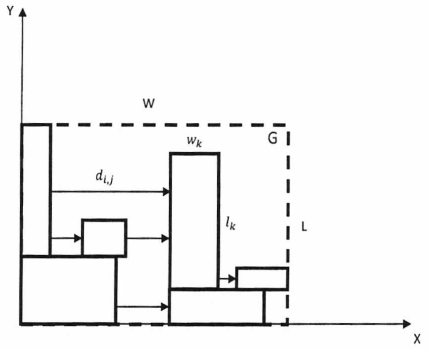
\includegraphics[scale=0.5]{diagram_prostokaty}
         \end{figure}
        
    \end{columns}
\end{frame}

\begin{frame}
    \frametitle{Algorytm pakowania}   
    Niech $\alpha=(r_1,r_2,\dots,r_n)$ będzie pewnym ciągiem prostokątów. Rozpatrujemy prostokąty
    zgodnie z kolejnością ich występowania w $\alpha$. Zbiór $P_{i-1}$ zawiera pozycje, na
    których można umieścić rozpatrywany prostokąt $r_i$.
    
    \begin{algorithmic}
        \State $G\gets\emptyset, P_0\gets\{(0,0)\}$
        \For{$i\gets 1, n$}
            \State $O\gets\emptyset$
            \For{$z$ in $P_{i-1}$} $O\gets O \cup \{insert(G, z, r_i)\}$\EndFor
            \State $G\gets$ wybrany na podstawie ustalonej strategii
            obszar z $O$ powstały po wstawieniu $r_i$ na pozycję $z=(x,y)$.
            \State $P_i\gets P_{i-1}\setminus\{z\}\cup\{(x+d_{r_c,r_i}\cdot\delta,y),
            (x+d_{r_c,r_i}\cdot\delta,y+l_i)\}$
        \EndFor
    \end{algorithmic}
    $\delta\in\{0,1\}$ i przyjmuje wartość 1, jeżeli wstawiany prostokąt $r_i$ został
    przesunięty o wielkość $d_{r_c,r_i}$, a pozycja $z$ została utworzona w wyniku
    wstawienia prostokąta $r_c$.
    
\end{frame}


\begin{frame}
    \frametitle{Strategie pakowania}
    \begin{enumerate}
        \item \textit{minimalnego obszaru} - wybierana jest pozycja, powodująca minimalne
        powiększenie bieżącego obszaru.
        \item \textit{pole-wymiary} - obliczana jest wartość współczynnika na podstawie pola
        powierzchni tymczasowego obszaru i różnicy długości jego boków. Zastosowanie
        tego współczynnika ma na celu tworzenie obszarów o równomiernym kształcie (zbliżonym
        do kwadratu).
        \item \textit{ruletki} - pozycja wstawienia prostokąta jest losowana zgodnie z zasadą
        ruletki. Prawdopodobieństwo wylosowania jest proporcjonalne do wielkości tymczasowego
        obszaru.
        \item \textit{XYZ} - pozycja jest losowana zgodnie z rozkładem jednostajnym.
    \end{enumerate}
\end{frame}
%------------------------------------------------
\section{First Section} % Sections can be created in order to organize your presentation into discrete blocks, all sections and subsections are automatically printed in the table of contents as an overview of the talk
%------------------------------------------------

\subsection{Subsection Example} % A subsection can be created just before a set of slides with a common theme to further break down your presentation into chunks

\begin{frame}
\frametitle{Paragraphs of Text}
Sed iaculis dapibus gravida. Morbi sed tortor erat, nec interdum arcu. Sed id lorem lectus. Quisque viverra augue id sem ornare non aliquam nibh tristique. Aenean in ligula nisl. Nulla sed tellus ipsum. Donec vestibulum ligula non lorem vulputate fermentum accumsan neque mollis.\\~\\

Sed diam enim, sagittis nec condimentum sit amet, ullamcorper sit amet libero. Aliquam vel dui orci, a porta odio. Nullam id suscipit ipsum. Aenean lobortis commodo sem, ut commodo leo gravida vitae. Pellentesque vehicula ante iaculis arcu pretium rutrum eget sit amet purus. Integer ornare nulla quis neque ultrices lobortis. Vestibulum ultrices tincidunt libero, quis commodo erat ullamcorper id.
\end{frame}

%------------------------------------------------

\begin{frame}
\frametitle{Bullet Points}
\begin{itemize}
\item Lorem ipsum dolor sit amet, consectetur adipiscing elit
\item Aliquam blandit faucibus nisi, sit amet dapibus enim tempus eu
\item Nulla commodo, erat quis gravida posuere, elit lacus lobortis est, quis porttitor odio mauris at libero
\item Nam cursus est eget velit posuere pellentesque
\item Vestibulum faucibus velit a augue condimentum quis convallis nulla gravida
\end{itemize}
\end{frame}

%------------------------------------------------

\begin{frame}
\frametitle{Blocks of Highlighted Text}
\begin{block}{Block 1}
Lorem ipsum dolor sit amet, consectetur adipiscing elit. Integer lectus nisl, ultricies in feugiat rutrum, porttitor sit amet augue. Aliquam ut tortor mauris. Sed volutpat ante purus, quis accumsan dolor.
\end{block}

\begin{block}{Block 2}
Pellentesque sed tellus purus. Class aptent taciti sociosqu ad litora torquent per conubia nostra, per inceptos himenaeos. Vestibulum quis magna at risus dictum tempor eu vitae velit.
\end{block}

\begin{block}{Block 3}
Suspendisse tincidunt sagittis gravida. Curabitur condimentum, enim sed venenatis rutrum, ipsum neque consectetur orci, sed blandit justo nisi ac lacus.
\end{block}
\end{frame}

%------------------------------------------------

\begin{frame}
\frametitle{Multiple Columns}
\begin{columns}[c] % The "c" option specifies centered vertical alignment while the "t" option is used for top vertical alignment

\column{.45\textwidth} % Left column and width
\textbf{Heading}
\begin{enumerate}
\item Statement
\item Explanation
\item Example
\end{enumerate}

\column{.5\textwidth} % Right column and width
Lorem ipsum dolor sit amet, consectetur adipiscing elit. Integer lectus nisl, ultricies in feugiat rutrum, porttitor sit amet augue. Aliquam ut tortor mauris. Sed volutpat ante purus, quis accumsan dolor.

\end{columns}
\end{frame}

%------------------------------------------------
\section{Second Section}
%------------------------------------------------

\begin{frame}
\frametitle{Table}
\begin{table}
\begin{tabular}{l l l}
\toprule
\textbf{Treatments} & \textbf{Response 1} & \textbf{Response 2}\\
\midrule
Treatment 1 & 0.0003262 & 0.562 \\
Treatment 2 & 0.0015681 & 0.910 \\
Treatment 3 & 0.0009271 & 0.296 \\
\bottomrule
\end{tabular}
\caption{Table caption}
\end{table}
\end{frame}

%------------------------------------------------

\begin{frame}
\frametitle{Theorem}
\begin{theorem}[Mass--energy equivalence]
$E = mc^2$
\end{theorem}
\end{frame}

%------------------------------------------------

\begin{frame}[fragile] % Need to use the fragile option when verbatim is used in the slide
\frametitle{Verbatim}
\begin{example}[Theorem Slide Code]
\begin{verbatim}
\begin{frame}
\frametitle{Theorem}
\begin{theorem}[Mass--energy equivalence]
$E = mc^2$
\end{theorem}
\end{frame}\end{verbatim}
\end{example}
\end{frame}

%------------------------------------------------

\begin{frame}
\frametitle{Figure}
Uncomment the code on this slide to include your own image from the same directory as the template .TeX file.
%\begin{figure}
%\includegraphics[width=0.8\linewidth]{test}
%\end{figure}
\end{frame}

%------------------------------------------------

\begin{frame}[fragile] % Need to use the fragile option when verbatim is used in the slide
\frametitle{Citation}
An example of the \verb|\cite| command to cite within the presentation:\\~

This statement requires citation \cite{p1}.
\end{frame}

%------------------------------------------------

\begin{frame}
\frametitle{References}
\footnotesize{
\begin{thebibliography}{99} % Beamer does not support BibTeX so references must be inserted manually as below
\bibitem[Smith, 2012]{p1} John Smith (2012)
\newblock Title of the publication
\newblock \emph{Journal Name} 12(3), 45 -- 678.
\end{thebibliography}
}
\end{frame}

%------------------------------------------------

\begin{frame}
\Huge{\centerline{The End}}
\end{frame}

%----------------------------------------------------------------------------------------

\end{document} 